\documentclass[11pt,a4paper]{article}
\usepackage[latin1]{inputenc}
\usepackage{amsmath}
\usepackage{xcolor}
\usepackage{amsfonts}
\usepackage{amssymb}
\usepackage{graphicx}
\usepackage{listings}
\usepackage[margin=0.5in]{geometry}
\usepackage{caption}
\usepackage{subcaption}
\DeclareGraphicsExtensions{.pdf,.png,.jpg}



\lstset{
	frame=single,
	breaklines=true,
	postbreak=\raisebox{0ex}[0ex][0ex]{\ensuremath{\color{red}\hookrightarrow\space}},
	basicstyle=\ttfamily\footnotesize
	}
	\lstdefinelanguage{numpy}{
		keywords = {
			and,del,from,not,while,
			as,elif,global,or,with,
			assert,else,if,pass,yield,
			break,except,import,print,
			class,exec,in, raise,continue,
			finally,is, return,def,for,
			lambda,try
			},
			morekeywords = {numpy,fft,mean}
			}

\author{Mohammad A.Raji, Alok Hota}
\title{Parallel matrix multiplication with CUDA}

\begin{document}
	\maketitle
	
	\section{Introduction}
A well known example of parallelization using the GPU is matrix multiplication. The serial version of this operation has a time complexity of $O(n^3)$, however with GPU parallelization, in general we can gain a time complexity of $O(N)$ assuming that we don't have GPU core limitations. 
	
	\section{Evaluation}
	We tested our implementations on a machine with four Xeon CPUs and an Nvidia Quadro FX3800 GPU with 192 cores. 
	
	For evaluation, the runtime of the serial and parallel implementations are compared. The values used for the matrix sizes in this comparison were 64, 128, 256, 512, 1024 and 2048. The test script used for generating the random matrices and running the two versions on them can be found at \texttt{./src/sgemm/test.sh}. The results are shown in Figure \ref{perf}.
	\begin{figure}
		\centering
		\begin{subfigure}[b]{0.45\textwidth}
			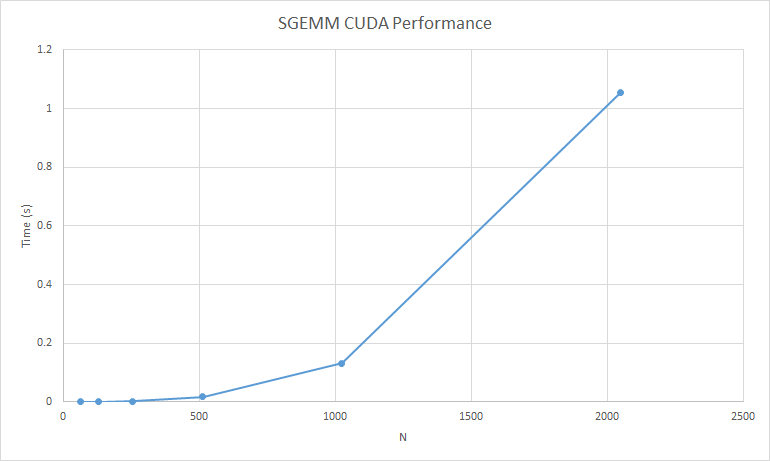
\includegraphics[width=\textwidth]{sgemm_cuda.png}
			\caption{Performance results for our parallel CUDA implementation}
			\label{nbody_cuda}
		\end{subfigure}
		\begin{subfigure}[b]{0.45\textwidth}
			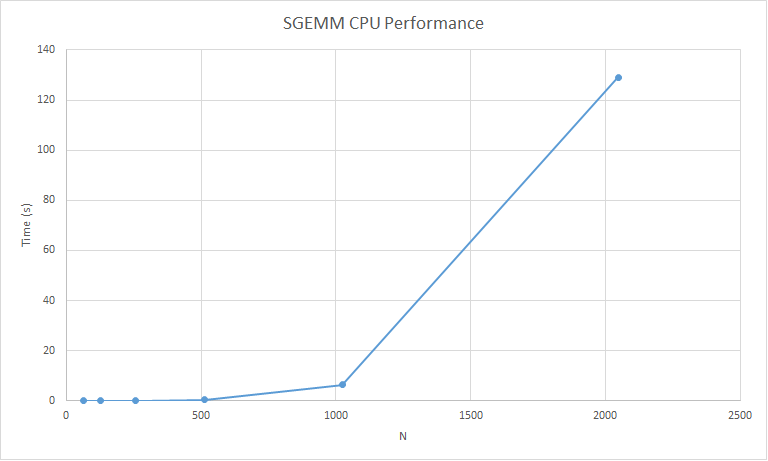
\includegraphics[width=\textwidth]{sgemm_cpu.png}
			\caption{Performance results for our serial implementation}
			\label{nbody_cpu}
		\end{subfigure}
		\caption{Performance comparison between our serial and parallel implementations}
		\label{perf}
	\end{figure}
	\pagebreak
	
	\section{Appendix A: Installation}
		The code for our work is available at http://github.com/ahota/nobody and can be downloaded using Git by running: \texttt{git clone http://github.com/ahota/nobody}.
		
		\subsection{Dependencies}
		For running the simulation, the only dependency is a machine with an Nvidia GPU that supports CUDA. 
		
		\subsection{Compiling}
		The serial and the parallel implementations can be compiled by running \texttt{./src/sgemm/compile.sh}. 
		
		\subsection{Running the simulation}
		For running the serial or the parallel versions, the user has to generate a random or an identity matrix. Matrices can be created using the gen\_matrix.py file. The usage of this script is as follows: 
		\\\\
		\texttt{python gen\_matrix.py [SIZE] [FILENAME] [TYPE]}
		\\\\
		where SIZE indicates the number of rows/columns, FILENAME is the output file's name and TYPE can be either -t for an identity matrix or -r for a random matrix.
		
		For the serial version, run \texttt{./src/sgemm/sgemm\_cpu}.
		The parallel version can be executed by running \texttt{./src/sgemm/sgemm\_cuda}. Both of these programs read the two input matrices from two files with the names of ``A.txt" and ``B.txt" and write the output to ``C.txt"
		
	\section{Appendix B: Header file}
	\begin{lstlisting}[language=c]
#include<stdio.h>
#include<stdlib.h>
#include<sys/time.h>
#include<time.h>

#define TILE_WIDTH_M 40
#define TILE_WIDTH_N 16
#define K TILE_WIDTH_M/TILE_WIDTH_N

__global__ void matrix_multiply_kernel(float *A, float *B, float *C,
int numARows, int numAColumns,
int numBRows, int numBColumns,
int numCRows, int numCColumns);
void matrix_multiply(float *A, float *B, float *C, int numARows,
int numAColumns, int numBRows, int numBColumns,
int numCRows, int numCColumns);
	\end{lstlisting}
	
	
	\section{Appendix B: Serial version}
	
	\begin{lstlisting}[language=c]
#include <stdio.h>
#include <stdlib.h>
#include <string.h>

typedef struct {
	struct timeval start;
	struct timeval end;
} timer;

void start_timer(timer *t) {
	gettimeofday( &(t->start), NULL);
}

void stop_timer(timer *t) {
	gettimeofday( &(t->end), NULL);
}

float elapsed_time(timer *t) {
	return (float) (t->end.tv_sec  - t->start.tv_sec)  + 
	(t->end.tv_usec - t->start.tv_usec) /
	1000000.0;
}

int main(int argc, char **argv) {
	float *A; // The A matrix
	float *B; // The B matrix
	float *C; // The output C matrix
	int numARows;    // number of rows in the matrix A
	int numAColumns; // number of columns in the matrix A
	int numBRows;    // number of rows in the matrix B
	int numBColumns; // number of columns in the matrix B
	int numCRows;    // number of rows in the matrix C (you have to set this)
	int numCColumns; // number of columns in the matrix C (you have to set this)
	char pathA[8] = "A.txt";
	char pathB[8] = "B.txt";
	char pathC[8] = "C.txt";
	timer perf_timer;
	timer total_timer;
	
	printf("Loading matrices...\n");
	
	start_timer(&total_timer);
	
	//load A and B
	FILE *file = fopen(pathA, "r");
	fscanf(file, "%d %d", &numARows, &numAColumns);
	A = (float *)malloc(numARows * numAColumns * sizeof(float));
	int r, c;
	for(r = 0; r < numARows; r++) {
		for(c = 0; c < numAColumns; c++) {
			fscanf(file, "%f", &A[r*numARows + c]);
		}
	}
	fclose(file);
	file = fopen(pathB, "r");
	fscanf(file, "%d %d", &numBRows, &numBColumns);
	B = (float *)malloc(numBRows * numBColumns * sizeof(float));
	for(r = 0; r < numBRows; r++) {
		for(c = 0; c < numBColumns; c++) {
			fscanf(file, "%f", &B[r*numBRows + c]);
		}
	}
	fclose(file);
	
	printf("Allocating memory...\n");
	
	numCRows = numAColumns; //Had to switch this because A is transposed
	numCColumns = numBColumns;
	C = ( float * )malloc(sizeof(float) * numCRows * numCColumns);
	
	printf("Calculating...\n");
	start_timer(&perf_timer);
	//multiply!
	int i;
	for(r = numAColumns - 1; r >= 0; r--) {
		for(c = 0; c < numBColumns; c++) {
			float sum = 0;
			for(i = 0; i < numARows; i++) {
				sum += A[r*numAColumns + i] * B[i*numBColumns + c];
			}
			C[r * numCRows + c] = sum;
		}
	}
	stop_timer(&perf_timer);
	
	printf("Saving result...\n");
	
	FILE *output = fopen(pathC, "w");
	fprintf(output, "%d %d\n", numCRows, numCColumns);
	for(r = 0; r < numCRows; r++) {
		for(c = 0; c < numCColumns; c++) {
			fprintf(output, "%.5f ", C[r*numCRows + c]);
		}
		fprintf(output, "\n");
	}
	fclose(output);
	stop_timer(&total_timer);
	
	printf("Calculation runtime = %f s\n", elapsed_time(&perf_timer));
	printf("Total runtime       = %f s\n", elapsed_time(&total_timer));
	
	
	return 0;
	
}
	\end{lstlisting}
	
	\section{Appendix C: Parallel version}
	
	\begin{lstlisting}[language=c]
#include "sgemm.h"

typedef struct {
	struct timeval start;
	struct timeval end;
} timer;

void start_timer(timer *t) {
	gettimeofday( &(t->start), NULL);
}

void stop_timer(timer *t) {
	gettimeofday( &(t->end), NULL);
}

float elapsed_time(timer *t) {
	return (float) (t->end.tv_sec  - t->start.tv_sec)  + 
	(t->end.tv_usec - t->start.tv_usec) /
	1000000.0;
}

// Compute C = A * B
__global__ void matrix_multiply_kernel(float *A, float *B, float *C,
int numARows, int numAColumns,
int numBRows, int numBColumns,
int numCRows, int numCColumns) {
	
	__shared__ float N_TILE[K][TILE_WIDTH_N]; //Tile for holding B elements
	int boffsetx = TILE_WIDTH_N * blockIdx.x; //block offsets
	int boffsety = TILE_WIDTH_M * blockIdx.y;
	
	int i, j, l;
	float slice[K]; //Current slice of row in A
	float out[TILE_WIDTH_N]; //Output to write to C after completing
	
	//Fill output with 0 so we can sum later
	for(i = 0; i < TILE_WIDTH_N; i++) {
		out[i] = 0;
	}
	
	//For each slice in our row
	for(i = 0; i < numARows; i += K) {
		//Load an element from B to our shared memory tile 
		N_TILE[threadIdx.x/TILE_WIDTH_N][threadIdx.x % TILE_WIDTH_N] =
		(threadIdx.x/TILE_WIDTH_N + i < numBRows &&
		threadIdx.x % TILE_WIDTH_N + boffsetx < numBColumns) ?
		B[boffsetx + numBColumns * (threadIdx.x / TILE_WIDTH_N + i)
		+ threadIdx.x  % TILE_WIDTH_N] : 0;
		
		//Load our slice to registers (if within bounds)
		if(threadIdx.x + boffsety < numCRows) {
			for(l = 0; l < K; ++l) {
				slice[l] = (i + l < numARows) ?
				A[boffsety + threadIdx.x + numAColumns * (l + i)] : 0;
			}
		}
		
		//Sync so every thread is using the correct values
		__syncthreads();
		
		//For every element across the shared memory tile
		for(l = 0; l < TILE_WIDTH_N; ++l) {
			//For each element in our slice
			for(j = 0; j < K; ++j) {
				out[l] += slice[j] * N_TILE[j][l];
			}
		}
	}
	
	//Write the results back to global memory (if within bounds)
	if(threadIdx.x + boffsety < numCRows) {
		for(i = 0; i < TILE_WIDTH_N; ++i) {
			if(boffsetx + i < numCColumns) {
				C[boffsetx + i + numCColumns * (boffsety + threadIdx.x)] =
				out[i];
			}
		}
	}
	
	//Sync so that we know every thread is done with the shared memory tile
	__syncthreads();
	
}

void matrix_multiply(float *A, float *B, float *C, int numARows,
int numAColumns, int numBRows, int numBColumns,
int numCRows, int numCColumns) {
	//launch matrix multiplication
	dim3 grid_size;
	int block_size;
	grid_size.x = ceil(numCColumns/float(TILE_WIDTH_N));
	grid_size.y = ceil(numCRows/float(TILE_WIDTH_M));
	block_size = TILE_WIDTH_M;
	
	matrix_multiply_kernel<<<grid_size, block_size>>>
	(A, B, C, numARows, numAColumns, numBRows, numBColumns,
	numCRows, numCColumns);
}

int main(int argc, char **argv) {
	float *hostA; // The A matrix
	float *hostB; // The B matrix
	float *hostC; // The output C matrix
	float *deviceA;
	float *deviceB;
	float *deviceC;
	int numARows;    // number of rows in the matrix A
	int numAColumns; // number of columns in the matrix A
	int numBRows;    // number of rows in the matrix B
	int numBColumns; // number of columns in the matrix B
	int numCRows;    // number of rows in the matrix C (you have to set this)
	int numCColumns; // number of columns in the matrix C (you have to set this)
	char pathA[8] = "A.txt";
	char pathB[8] = "B.txt";
	char pathC[8] = "C.txt";
	timer perf_timer;
	timer total_timer;
	
	//load A and B
	printf("Loading matrices...\n");
	
	start_timer(&total_timer);
	FILE *file = fopen(pathA, "r");
	fscanf(file, "%d %d", &numARows, &numAColumns);
	hostA = (float *)malloc(numARows * numAColumns * sizeof(float));
	int r, c;
	for(r = 0; r < numARows; r++) {
		for(c = 0; c < numAColumns; c++) {
			fscanf(file, "%f", &hostA[r*numARows + c]);
		}
	}
	fclose(file);
	file = fopen(pathB, "r");
	fscanf(file, "%d %d", &numBRows, &numBColumns);
	hostB = (float *)malloc(numBRows * numBColumns * sizeof(float));
	for(r = 0; r < numBRows; r++) {
		for(c = 0; c < numBColumns; c++) {
			fscanf(file, "%f", &hostB[r*numBRows + c]);
		}
	}
	fclose(file);
	
	printf("Allocating memory...\n");
	
	numCRows = numAColumns; //Had to switch this because A is transposed
	numCColumns = numBColumns;
	hostC = ( float * )malloc(sizeof(float) * numCRows * numCColumns);
	
	cudaMalloc((void**) &deviceA, sizeof(float) * numARows * numAColumns);
	cudaMalloc((void**) &deviceB, sizeof(float) * numBRows * numBColumns);
	cudaMalloc((void**) &deviceC, sizeof(float) * numCRows * numCColumns);
	
	printf("Copying to device...\n");
	
	cudaMemcpy(deviceA, hostA, sizeof(float) * numARows * numAColumns,
	cudaMemcpyHostToDevice);
	cudaMemcpy(deviceB, hostB, sizeof(float) * numBRows * numBColumns,
	cudaMemcpyHostToDevice);
	
	printf("Running kernel...\n");
	
	start_timer(&perf_timer);
	matrix_multiply(deviceA, deviceB, deviceC, numARows, numAColumns, numBRows,
	numBColumns, numCRows, numCColumns);
	cudaDeviceSynchronize();
	stop_timer(&perf_timer);
	
	printf("Copying back...\n");
	
	cudaMemcpy(hostC, deviceC, sizeof(float) * numCRows * numCColumns,
	cudaMemcpyDeviceToHost);
	
	printf("Saving result...\n");
	
	//print C
	FILE *output = fopen(pathC, "w");
	fprintf(output, "%d %d\n", numCRows, numCColumns);
	for(r = 0; r < numCRows; r++) {
		for(c = 0; c < numCColumns; c++) {
			fprintf(output, "%.5f ", hostC[r*numCRows + c]);
		}
		fprintf(output, "\n");
	}
	fclose(output);
	
	cudaFree(deviceA);
	cudaFree(deviceB);
	cudaFree(deviceC);
	
	stop_timer(&total_timer);
	printf("Kernel runtime = %f s\n", elapsed_time(&perf_timer));
	printf("Total runtime  = %f s\n", elapsed_time(&total_timer));
	
	printf("Done.\n");
	
	return 0;
}

\end{lstlisting}
	
\end{document}
